% PDF link
\documentclass[../structure.tex]{subfiles}
\begin{document}

\chapter{implementation}
To implement the method we have discussed before, we wrote the code in \textit{Python Programming Language} and \textit{Spyder} version 3 and \textit{Integrated Development Environment (IDE)} are used.

As we mentioned before, our data is in \textit{\textbf{ply}} format as shown in figure \{\ref{fig:data}\}, to read this format we wrote our own method using \textit{plyfile} library due to special case of our data which has different arrangement files. The method we wrote return data in \textit{numpy ndarray} structure where each array tract is putted in an array and all tracts belong to the same bundle were putted together with respect to the sequences of the neighboring vertices.

Then we apply PCA transformation (\textit{sklearn.decomposition} library) to the data and generate histogram (\textit{matplotlib.pyplot} library) for distances between each vertex in the template graph $S$ and its closet vertex in target graph $T$, before and after PCA transformation to compare the distance difference, because in some cases where the two graphs (template and target) are already in the best alignment before ICP, PCA transformation increase the distance between them as we will show in the result chapter. If the distance between two graphs is increased we drop the PCA transformation step. For distance measurement we use \textit{K-D tree} from \textit{scikit learn}.

We continue to build variables as shown in equation (\ref{equ:finalCostFun}), to do so, we use histograms generated in the previous step to determine the threshold for the maximum distance we need to consider for $W$ in the \textbf{distance term} for cost function, if the value is equal or below the threshold $w_{i} = 1$, otherwise $w_{i} = 0$. Then we build $W$ as diaginal sparse matrix using \textit{scipy.sparse} library. Then we continue using the same library (\textit{scipy.sparse}) to build $D$ sparse matrix and calculate $WD$ and $WU$.

Now we have \textbf{the distance term} of the cost function, we need to build the \textbf{stiffness term}, we use the same library (\textit{scipy.sparse}) to build $M$ sparse matrix and $G$ diagonal sparse matrix and calculate Kronecker product ($M\otimes G$).

The final step of building the cost function is to vertically stack $MG$ and $WD$ to have $A$, and vertically stack \textit{zero} sparse matrix and $WU$ to have $B$ as require $||Ax-b||_{F}^2$.

The last step is solving the cost fuction $||Ax-b||_{F}^2$ by using \textbf{\textit{LSQR}} from \textit{scipy.sparse.linalg} library. As mentioned in the \textit{scipy.sparse.linalg.lsqr} documentation \cite{Jones2001}, $b$ in equation $Ax-b$ must be a vector, and as $b$ in our case is a matrix size $n\times 3$, we use matrices fundamental concept to solve this problem as we use \textbf{lsqrt} three times for each column and horizontally stack the result to get the affine matrices combination.

Finally for visualization we customize functions from \textit{open3d} library to view brain bundles due to special case of our data.


\begin{figure}[h!]
\centering
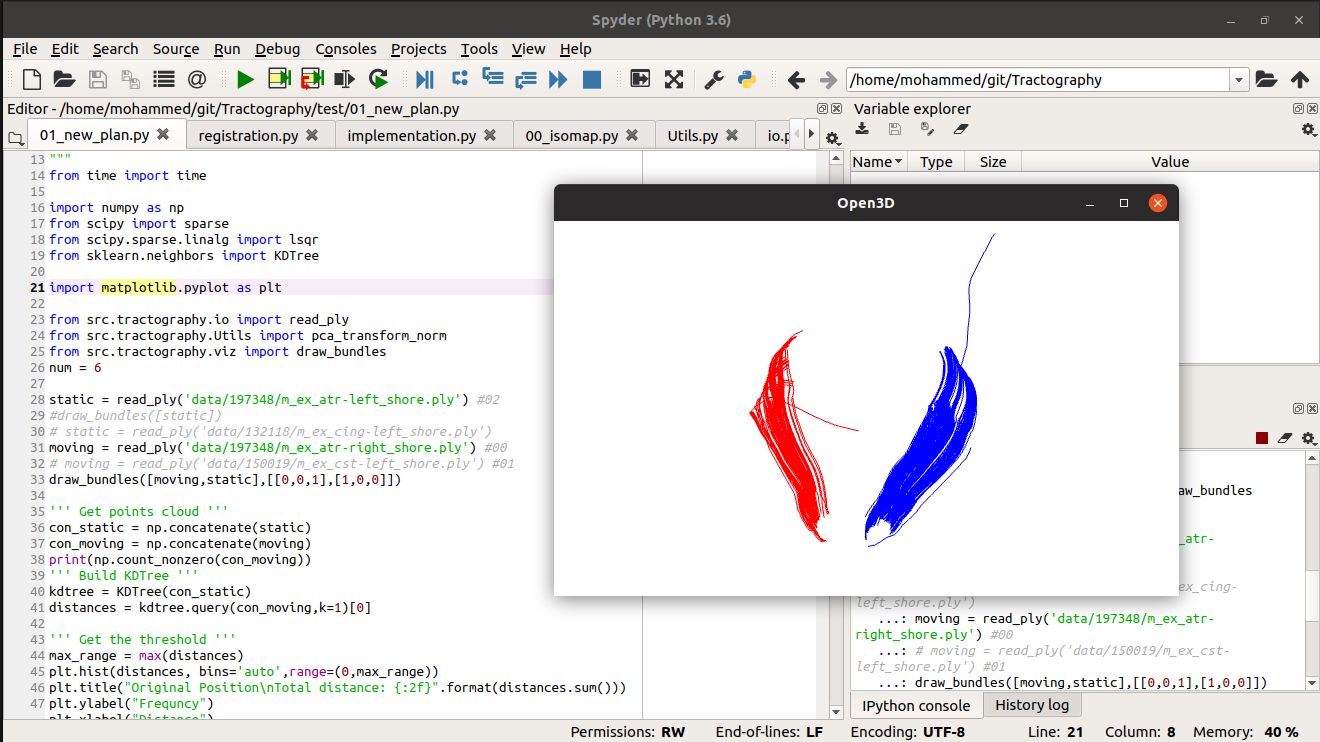
\includegraphics[scale=0.3]{008_ide}
\captionsetup{justification=centering}
\caption{IDE and visualization tool}
\end{figure}

\end{document}

